\subsection{UC3: Autenticazione standard}
    \label{sec:UC3}
    \begin{figure}[!ht]
        \caption{Diagramma di UC3: Autenticazione standard}
        \vspace{10px}
        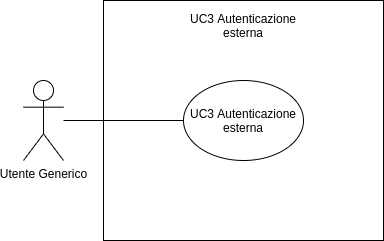
\includegraphics[scale=0.5]{../../../Images/AnalisiRequisiti/UC03}
        \centering
    \end{figure}
    \begin{itemize}
        \item \textbf{Descrizione:} permette l'autenticazione di un utente;
        \item \textbf{Attore Primario:} utente generico;
        \item \textbf{Attore Secondario:} Amazon Cognito;
        \item \textbf{Precondizione:} l'utente generico non si è ancora autenticato
        \item \textbf{Input:} pressione bottone login;
        \item \textbf{Postcondizione:} l'utente è autenticato;
        \item \textbf{Scenario Principale:} 
        \begin{itemize}
            \item l'utente entra nella pagina
            \item preme il bottone per il login
            \item viene inderizzato alla pagina di login fornita da \textit{Amazon Cognito}.
        \end{itemize}
    \end{itemize}
